\documentclass[11pt,a4paper]{article}

% =========================================================
%  ASR STUDIO - PROJECT REPORT  (Overleaf ready, pdfLaTeX)
%  Upload this file + the figures/ folder + srm_logo.png
%  Every image is optional: if a file is missing, a framed
%  placeholder box is printed instead, so it always compiles.
% =========================================================

% ---------- Packages ----------
\usepackage[margin=0.9in]{geometry}
\usepackage{times}
\usepackage[T1]{fontenc}
\usepackage[utf8]{inputenc}
\usepackage{graphicx}
\usepackage{array}
\usepackage{tabularx}
\usepackage{longtable}
\usepackage{booktabs}
\usepackage{enumitem}
\usepackage[table]{xcolor}
\usepackage{listings}
\usepackage{tikz}
\usetikzlibrary{positioning,arrows.meta,shapes.misc,shapes.geometric,fit,calc}
\usepackage{setspace}
\usepackage{titlesec}
\usepackage{fancyhdr}
\usepackage{caption}
\usepackage{float}
\usepackage{amsmath,amssymb}
\usepackage[colorlinks=true,linkcolor=black,urlcolor=blue]{hyperref}

\setstretch{1.02}
\setlength{\parindent}{0pt}
\setlength{\parskip}{6pt}

% ---------- Colours ----------
\definecolor{emerald}{HTML}{10B981}
\definecolor{headblue}{HTML}{1F3A8A}
\definecolor{rowgray}{HTML}{F4F6FA}
\definecolor{codebg}{HTML}{F5F5F5}

% ---------- Headings (UPPERCASE, numbered like the reference) ----------
\titleformat{\section}{\large\bfseries}{\thesection.}{0.5em}{\MakeUppercase}
\titleformat{\subsection}{\normalsize\bfseries}{\thesubsection}{0.6em}{}
\titlespacing*{\section}{0pt}{6pt}{6pt}
\titlespacing*{\subsection}{0pt}{8pt}{4pt}

% ---------- Header / footer ----------
\pagestyle{fancy}
\fancyhf{}
\fancyhead[L]{\small ASR Studio Project Report}
\fancyhead[R]{\small SRM IST, Tiruchirappalli}
\fancyfoot[C]{\small\thepage}
\renewcommand{\headrulewidth}{0.4pt}
\setlength{\headheight}{15pt}

% ---------- Table helpers ----------
\newcolumntype{L}[1]{>{\raggedright\arraybackslash}p{#1}}
\newcolumntype{Y}{>{\raggedright\arraybackslash}X}
\newcommand{\thc}[1]{\textcolor{white}{\bfseries #1}}
\newcommand{\headrow}{\rowcolor{headblue}}
\renewcommand{\arraystretch}{1.35}

% ---------- Optional figure helper ----------
% \screenshot{file}{width}{caption}
\newcommand{\screenshot}[3]{%
\begin{figure}[H]
\centering
\IfFileExists{#1}{%
  \fbox{\includegraphics[width=#2]{#1}}%
}{%
  \fbox{\parbox[c][5cm][c]{#2}{\centering\small\itshape Screenshot placeholder\\ (upload \texttt{#1})}}%
}
\caption{#3}
\end{figure}}

% ---------- Code listing styles ----------
\lstdefinestyle{base}{
  basicstyle=\ttfamily\footnotesize,
  backgroundcolor=\color{codebg},
  frame=single,
  rulecolor=\color{gray!50},
  breaklines=true,
  showstringspaces=false,
  columns=fullflexible,
  keepspaces=true,
  keywordstyle=\color{headblue}\bfseries,
  commentstyle=\color{gray}\itshape,
  stringstyle=\color{emerald!60!black}
}
\lstdefinestyle{json}{style=base}
\lstdefinestyle{py}{style=base,language=Python}
\lstdefinestyle{sh}{style=base,language=bash}

\captionsetup{font=small,labelfont=it,textfont=it}

\begin{document}

%==================================================
% COVER PAGE
%==================================================
\begin{titlepage}
\centering
\vspace*{0.2cm}

{\LARGE\bfseries ASR STUDIO: AN END-TO-END AUTOMATIC SPEECH RECOGNITION STUDIO USING OPENAI WHISPER, FASTAPI AND REACT (NODE.JS)}\\[10pt]
{\normalsize\bfseries On-Device Faster-Whisper Inference, Voice Activity Detection, Multi-Format Subtitle Export and Batch Processing}\\[22pt]

{\large\bfseries A PROJECT REPORT}\\[18pt]

{\itshape Submitted by}\\[6pt]
{\bfseries KARTHIG RAJAN [Reg No: RA2311003050204]}\\
{\bfseries SACHIN KUPPUSWAMY [Reg No: RA2311003050263]}\\
{\bfseries NANDAKISHORE K S [Reg No: RA2311003050216]}\\[16pt]

{\itshape Under the guidance of}\\[6pt]
{\large\bfseries Dr. R. Baskar}\\
(Assistant Professor, Department of Computer Science \& Engineering)\\[14pt]

in partial fulfilment of the requirements for the degree of\\[2pt]
{\bfseries BACHELOR OF TECHNOLOGY}\\
in\\
{\bfseries COMPUTER SCIENCE AND ENGINEERING}\\[0.6cm]

\IfFileExists{srm_logo.png}{%
  \includegraphics[width=5cm]{srm_logo.png}\par
}{%
  {\Huge\bfseries\color{blue!50!black} SRM}\\[2pt]
  {\small\colorbox{blue!50!black}{\color{white} TIRUCHIRAPPALLI}}\par
}
\vspace{0.6cm}

{\bfseries DEPARTMENT OF COMPUTER SCIENCE AND ENGINEERING}\\
{\bfseries FACULTY OF ENGINEERING AND TECHNOLOGY}\\
{\bfseries SRM INSTITUTE OF SCIENCE AND TECHNOLOGY}\\
{\bfseries TIRUCHIRAPPALLI -- 621105}\\
{\bfseries OCTOBER 2026}
\end{titlepage}

%==================================================
% TABLE OF CONTENTS
%==================================================
\begin{center}
{\Large\bfseries TABLE OF CONTENTS}
\end{center}
\vspace{4pt}
\renewcommand{\contentsname}{}
\vspace{-1.2cm}
\setcounter{tocdepth}{1}
\tableofcontents
\thispagestyle{fancy}

%==================================================
% AI DECLARATION (kept from the original report)
%==================================================
\clearpage
\section*{AI / LLM DECLARATION}
\addcontentsline{toc}{section}{AI / LLM Declaration}
I/We used Gemini / Claude (Gemini 3.7 / Claude 3.7) to assist in architecting the audio preprocessing workflow, structuring OpenAPI endpoint documentation, optimizing PyTest unit test coverage, and designing CSS design tokens for the Emerald Matrix UI theme.

The extent of AI/LLM usage is approximately 15--20\%, limited to architectural suggestions, documentation formatting, and visual layout references.

All core backend implementation logic, CTranslate2 Faster-Whisper model inference orchestration, audio signal resampling buffers, subtitle exporter serialization, CLI parser development, React component engineering, and end-to-end integration were done manually by the team.

\vspace{10pt}
\section*{PROJECT DETAILS AT A GLANCE}
\addcontentsline{toc}{section}{Project Details at a Glance}
\begin{tabularx}{\textwidth}{|>{\bfseries}L{4.2cm}|Y|}
\hline
Project Title & Automatic Speech Recognition (ASR) Studio \\ \hline
Team Members & Karthig Rajan (RA2311003050204), Sachin Kuppuswamy (RA2311003050263), Nandakishore K S (RA2311003050216) \\ \hline
Guide & Dr. R. Baskar, Assistant Professor, Dept. of CSE \\ \hline
Course & Modern Application Development \\ \hline
Frontend & React 19 + Vite (Node.js), Lucide icons, HTML5 Web Audio API \\ \hline
Backend & Python 3.10+, FastAPI, Uvicorn \\ \hline
ASR Core & Faster-Whisper (CTranslate2, int8) with SpeechRecognition fallback \\ \hline
Repository & \url{https://github.com/Rajan3103/asr-studio} \\ \hline
\end{tabularx}

%==================================================
% 1. EXECUTIVE SUMMARY + 2. INTRODUCTION
%==================================================
\clearpage
\section{Executive Summary}
ASR Studio is an end-to-end, browser-based Automatic Speech Recognition (ASR) platform that converts spoken audio into accurate, timestamped text. Users can either record their voice live through the browser microphone or upload pre-recorded audio files in WAV, MP3, FLAC, M4A, AAC and OGG formats. The audio is sent to a FastAPI microservice, where it is processed by Faster-Whisper, a CTranslate2-optimised re-implementation of OpenAI's Whisper transformer model, running with 8-bit integer (int8) quantisation on a standard CPU.

The system returns the full transcript, the detected language with its probability, per-segment start/end timestamps, a confidence score for every segment, and optional word-level timestamps. In addition to transcription, the same model can translate speech from more than 90 languages directly into English. Results can be copied in one click or downloaded as plain text (.txt), SubRip subtitles (.srt), WebVTT captions (.vtt), structured JSON (.json) or spreadsheet-ready CSV (.csv).

Around this core, the studio provides a synthetic-audio latency benchmark, a multi-file batch processing queue with live progress, an interactive REST API reference, a command-line interface (CLI) for scripted and directory-level transcription, and five switchable visual themes. The primary recognition path runs entirely on the user's own machine, so recorded speech is never sent to a paid cloud API, and the whole code base is covered by an automated suite of 20 PyTest unit and integration tests.

\section{Introduction \& Background}
Speech is the most natural way humans communicate, yet most digital systems still depend on typed text for search, documentation and accessibility. Automatic Speech Recognition bridges this gap by converting an acoustic signal into a sequence of words. Classical ASR systems were built from separately trained components: an acoustic model (often Gaussian Mixture Models or Hidden Markov Models), a pronunciation lexicon and an n-gram language model. These pipelines needed large amounts of hand-aligned data for every language and were fragile in the presence of accents, background noise and domain-specific vocabulary.

The arrival of deep learning, and in particular the Transformer architecture (Vaswani et al., 2017), changed this landscape. In 2022 OpenAI released Whisper, an encoder--decoder Transformer trained on 680,000 hours of weakly supervised multilingual audio. Whisper performs transcription, language identification and speech translation with a single network and is robust to noise and accents. However, the reference PyTorch implementation is heavy for ordinary laptops. Faster-Whisper re-implements Whisper on top of the CTranslate2 inference engine, which supports int8 quantisation and optimised CPU kernels, making on-device transcription practical without a GPU.

Commercial services such as Google Cloud Speech-to-Text, AWS Transcribe and Otter.ai offer high accuracy but require uploading audio to third-party servers and charge per minute of audio. For students, researchers and institutions handling lectures, interviews or confidential meetings, this raises privacy and cost concerns. ASR Studio was built to show that a modern web stack (React + FastAPI) combined with an optimised open-source model can deliver a polished, privacy-respecting transcription and captioning tool that runs on everyday hardware.

%==================================================
% 3. PROBLEM STATEMENT + 4. OBJECTIVES
%==================================================
\section{Problem Statement \& Motivation}
\textbf{Problem Statement:} To design and develop a high-performance, browser-based Automatic Speech Recognition (ASR) Studio that allows users to capture live voice via browser Web Audio APIs or upload multi-format audio files (WAV, MP3, FLAC, M4A, AAC, OGG) and receive accurate speech-to-text transcriptions, translation to English, and millisecond-level timed subtitle segments, with the primary inference path running fully on-device without paid cloud API dependencies.

Current deficiencies in everyday transcription and captioning workflows include:
\begin{itemize}[leftmargin=1.2em]
  \item \textbf{Cloud Privacy Risks:} Popular transcription services upload raw audio to external servers. Lectures, interviews, medical notes or internal meetings may contain sensitive information that should not leave the organisation.
  \item \textbf{Recurring Per-Minute Costs:} Cloud ASR APIs are billed per minute of audio. Departments that transcribe many hours of lectures every week face continuous operational expense.
  \item \textbf{Unstructured Output:} Many simple dictation tools return a single block of text without timestamps, which is useless for creating subtitles or locating a moment in a long recording.
  \item \textbf{Fragmented Tooling:} Recording, format conversion, transcription and subtitle generation are usually done in separate applications, forcing users to move files between tools.
  \item \textbf{Hardware Barrier:} The original Whisper implementation runs slowly on CPU-only laptops, which are the most common hardware available to students.
  \item \textbf{No Single-Point Failure Handling:} If a local model fails to load (for example, due to insufficient memory), most tools simply crash instead of degrading gracefully.
\end{itemize}

\section{Project Objectives \& Scope}
ASR Studio was engineered to fulfil the following objectives:
\begin{itemize}[leftmargin=1.2em]
  \item[$\blacksquare$] \textbf{On-Device Inference:} Run Whisper models locally through Faster-Whisper with int8 CPU quantisation so that the primary path needs no paid cloud API.
  \item[$\blacksquare$] \textbf{Flexible Audio Ingestion:} Accept live microphone recordings and six common audio formats, and normalise them into 16\,kHz mono float32 signals.
  \item[$\blacksquare$] \textbf{Rich, Structured Results:} Return transcript text, detected language, language probability, audio duration, processing time, timed segments, confidence and word timestamps.
  \item[$\blacksquare$] \textbf{Multi-Format Export:} Generate TXT, SRT, VTT, JSON and CSV outputs that can be used directly in video editors, media players and spreadsheets.
  \item[$\blacksquare$] \textbf{Configurable Inference:} Let the user choose model tier (tiny to large-v3), task (transcribe/translate), source language, beam size, VAD filtering and word timestamps.
  \item[$\blacksquare$] \textbf{Resilience:} Fall back automatically to a secondary SpeechRecognition engine if the Whisper model cannot run.
  \item[$\blacksquare$] \textbf{Multiple Interfaces:} Expose the same engine through a React web studio, a documented REST API and a command-line tool.
  \item[$\blacksquare$] \textbf{Quality Assurance:} Validate every module with automated PyTest unit and integration tests.
\end{itemize}

\textbf{Scope.} The project covers single-user transcription of recorded or uploaded audio, translation into English, subtitle generation and batch processing. Real-time word-by-word streaming, speaker diarisation (``who spoke when'') and user accounts/persistent storage are outside the current scope and are listed as future enhancements.

%==================================================
% 5. KEY FEATURES
%==================================================
\section{Key Features \& Specifications}
\subsection{Audio Capture \& Ingestion}
\begin{itemize}[leftmargin=1.2em,itemsep=1pt]
  \item Drag-and-drop or click-to-browse upload supporting WAV, MP3, FLAC, M4A, AAC and OGG.
  \item Live microphone recording through \texttt{navigator.mediaDevices.getUserMedia} and the \texttt{MediaRecorder} API, with a running recording timer.
  \item Real-time frequency-bar visualiser drawn on an HTML5 canvas using a Web Audio \texttt{AnalyserNode} (FFT size 128).
  \item Automatic audio signal analysis on selection: duration, sample rate, RMS energy, peak amplitude and silence detection.
\end{itemize}

\subsection{Speech Recognition Engine}
\begin{itemize}[leftmargin=1.2em,itemsep=1pt]
  \item Faster-Whisper (CTranslate2) with int8 quantisation running on CPU by default, CUDA optional through the CLI.
  \item Five model tiers: \texttt{tiny}, \texttt{base} (default), \texttt{small}, \texttt{medium}, \texttt{large-v3}.
  \item Transcribe mode (same language) and Translate mode (any supported language $\rightarrow$ English).
  \item Automatic language detection or manual selection among 15 commonly used languages in the UI (Whisper itself supports 90+).
  \item Silero Voice Activity Detection (VAD) filter to skip silent and non-speech regions.
  \item Configurable beam search width (1--10) and word-level timestamps.
  \item Model instances are cached per tier, so the model is loaded from disk only once per server lifetime.
  \item Automatic fallback to the SpeechRecognition library if Faster-Whisper raises an error.
\end{itemize}

\subsection{Results Viewer \& Export Hub}
\begin{itemize}[leftmargin=1.2em,itemsep=1pt]
  \item Full transcript panel with one-click copy to clipboard.
  \item Metadata cards: detected language, language probability, audio duration, processing time and engine used.
  \item Timed segments inspector listing start/end time, text and confidence for every segment.
  \item One-click download in five formats: TXT, SRT, VTT, JSON and CSV.
\end{itemize}

\subsection{Productivity \& Developer Tools}
\begin{itemize}[leftmargin=1.2em,itemsep=1pt]
  \item \textbf{Synthetic Benchmark:} generates a 1--10 second harmonic test signal and measures end-to-end pipeline latency.
  \item \textbf{Batch Queue:} upload several files and process them sequentially with a live progress bar.
  \item \textbf{REST API \& CLI Docs tab:} in-app reference with ready-to-copy \texttt{curl} and CLI commands; interactive Swagger UI at \texttt{/docs}.
  \item \textbf{Theme Engine:} five themes -- Emerald Matrix / Dark Velvet, Cyber Obsidian, Deep Nebula, Tokyo Sunset and Nordic Frost.
\end{itemize}

%==================================================
% 6. ARCHITECTURE
%==================================================
\clearpage
\section{System Architecture \& High-Level Design}
ASR Studio follows a decoupled client--server architecture. The React single-page application handles all user interaction and talks to the Python backend exclusively through HTTP requests with multipart form-data payloads. The backend is organised as a pipeline of small, single-purpose modules that can also be reused independently by the command-line tool.

\begin{figure}[H]
\centering
\resizebox{\textwidth}{!}{%
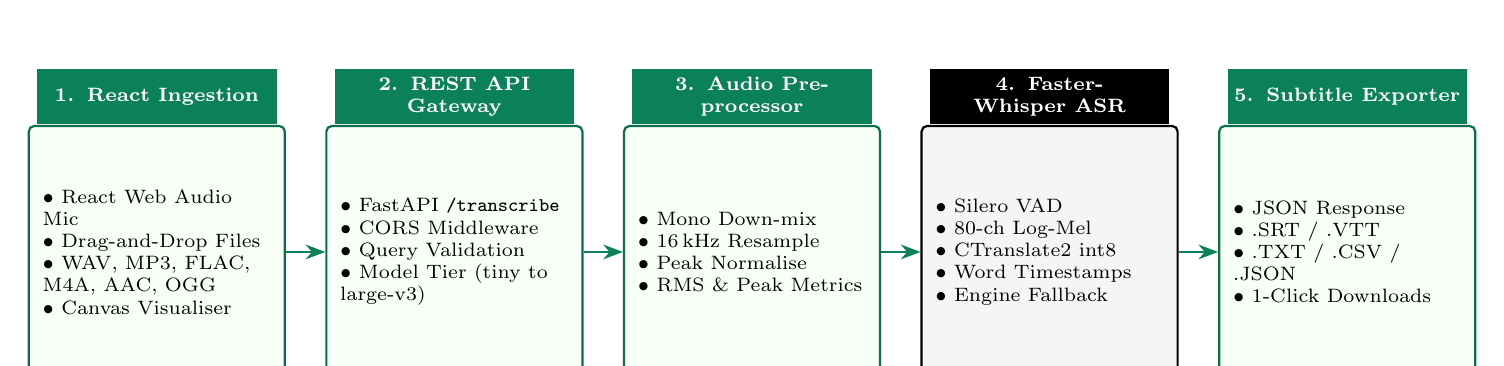
\begin{tikzpicture}[
  stage/.style={draw=emerald!60!black, thick, rectangle, rounded corners=2pt,
                text width=2.9cm, minimum height=3.2cm, align=left,
                font=\scriptsize, fill=green!3, inner sep=5pt},
  head/.style={font=\scriptsize\bfseries, text=white, fill=emerald!70!black,
               text width=2.9cm, align=center, minimum height=0.7cm, inner sep=2pt},
  arr/.style={-{Stealth[length=2.5mm]}, thick, emerald!70!black}
]
\node[stage] (s1) {$\bullet$ React Web Audio Mic\\$\bullet$ Drag-and-Drop Files\\$\bullet$ WAV, MP3, FLAC, M4A, AAC, OGG\\$\bullet$ Canvas Visualiser};
\node[head, anchor=south] at (s1.north) {1. React Ingestion};
\node[stage, right=0.5cm of s1] (s2) {$\bullet$ FastAPI \texttt{/transcribe}\\$\bullet$ CORS Middleware\\$\bullet$ Query Validation\\$\bullet$ Model Tier (tiny to large-v3)};
\node[head, anchor=south] at (s2.north) {2. REST API Gateway};
\node[stage, right=0.5cm of s2] (s3) {$\bullet$ Mono Down-mix\\$\bullet$ 16\,kHz Resample\\$\bullet$ Peak Normalise\\$\bullet$ RMS \& Peak Metrics};
\node[head, anchor=south] at (s3.north) {3. Audio Preprocessor};
\node[stage, right=0.5cm of s3, draw=black, fill=gray!8] (s4) {$\bullet$ Silero VAD\\$\bullet$ 80-ch Log-Mel\\$\bullet$ CTranslate2 int8\\$\bullet$ Word Timestamps\\$\bullet$ Engine Fallback};
\node[head, anchor=south, fill=black] at (s4.north) {4. Faster-Whisper ASR};
\node[stage, right=0.5cm of s4] (s5) {$\bullet$ JSON Response\\$\bullet$ .SRT / .VTT\\$\bullet$ .TXT / .CSV / .JSON\\$\bullet$ 1-Click Downloads};
\node[head, anchor=south] at (s5.north) {5. Subtitle Exporter};
\draw[arr] (s1) -- (s2);
\draw[arr] (s2) -- (s3);
\draw[arr] (s3) -- (s4);
\draw[arr] (s4) -- (s5);
\end{tikzpicture}}
\caption{End-to-end system architecture and audio pipeline of ASR Studio}
\end{figure}

\begin{tabularx}{\textwidth}{|L{3.3cm}|L{4.6cm}|Y|}
\hline
\headrow \thc{Architectural Tier} & \thc{Components \& Technologies} & \thc{Core Responsibilities} \\ \hline
\textbf{Tier 1: Presentation \& Audio Ingestion} & React 19, Vite, Lucide icons, Web Audio API, MediaRecorder, Canvas & File upload, live recording, visualiser, model configuration, results viewer, theme switching \\ \hline
\textbf{Tier 2: REST API Gateway} & FastAPI, Uvicorn, python-multipart, CORS middleware & Endpoint routing, enum-based query validation, temporary file handling, error mapping to HTTP 400/500 \\ \hline
\textbf{Tier 3: Signal Processing} & SoundFile, SciPy \texttt{signal.resample}, NumPy, \texttt{wave} & Decoding, mono conversion, 16\,kHz resampling, normalisation, metrics, synthetic signal generation \\ \hline
\textbf{Tier 4: ASR Inference} & Faster-Whisper, CTranslate2, Silero VAD, SpeechRecognition & Model caching, transcription, translation, language detection, timestamps, confidence, fallback \\ \hline
\textbf{Tier 5: Serialisation \& Export} & \texttt{json}, \texttt{csv}, custom timecode formatter & TXT/SRT/VTT/JSON/CSV generation and file streaming with \texttt{Content-Disposition} headers \\ \hline
\end{tabularx}

\subsection{Request Sequence for a Transcription}
\begin{figure}[H]
\centering
\resizebox{0.95\textwidth}{!}{%
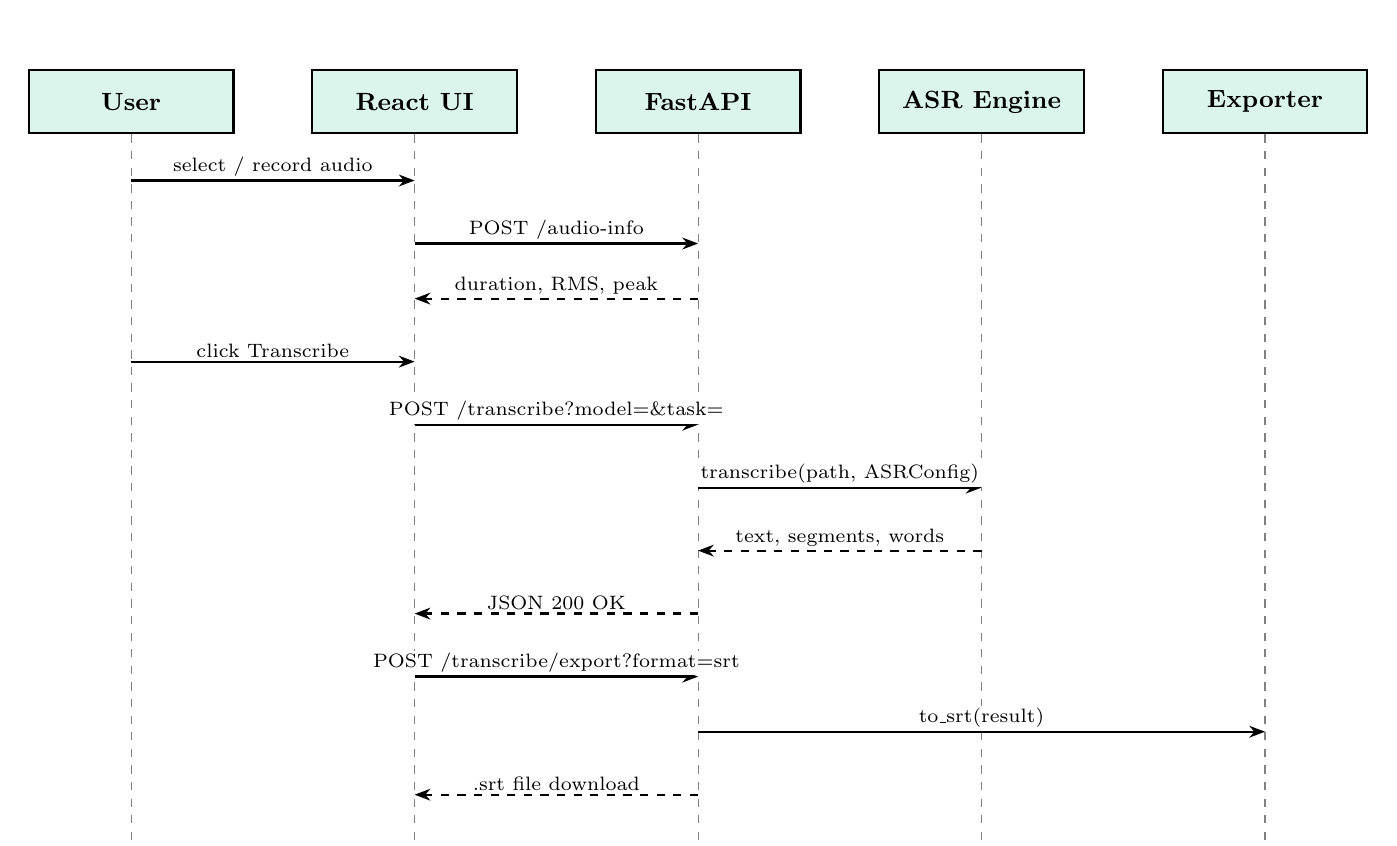
\begin{tikzpicture}[
  actor/.style={draw, thick, fill=emerald!15, minimum width=2.6cm, minimum height=0.8cm, font=\small\bfseries},
  msg/.style={-{Stealth[length=2mm]}, thick},
  ret/.style={-{Stealth[length=2mm]}, thick, dashed},
  lbl/.style={font=\scriptsize, fill=white, inner sep=1pt}
]
\node[actor] (u) at (0,0) {User};
\node[actor] (r) at (3.6,0) {React UI};
\node[actor] (a) at (7.2,0) {FastAPI};
\node[actor] (e) at (10.8,0) {ASR Engine};
\node[actor] (x) at (14.4,0) {Exporter};
\foreach \n in {u,r,a,e,x} { \draw[gray, dashed] (\n.south) -- ++(0,-9.2); }
\draw[msg] (0,-1.0) -- node[lbl,above]{select / record audio} (3.6,-1.0);
\draw[msg] (3.6,-1.8) -- node[lbl,above]{POST /audio-info} (7.2,-1.8);
\draw[ret] (7.2,-2.5) -- node[lbl,above]{duration, RMS, peak} (3.6,-2.5);
\draw[msg] (0,-3.3) -- node[lbl,above]{click Transcribe} (3.6,-3.3);
\draw[msg] (3.6,-4.1) -- node[lbl,above]{POST /transcribe?model=\&task=} (7.2,-4.1);
\draw[msg] (7.2,-4.9) -- node[lbl,above]{transcribe(path, ASRConfig)} (10.8,-4.9);
\draw[ret] (10.8,-5.7) -- node[lbl,above]{text, segments, words} (7.2,-5.7);
\draw[ret] (7.2,-6.5) -- node[lbl,above]{JSON 200 OK} (3.6,-6.5);
\draw[msg] (3.6,-7.3) -- node[lbl,above]{POST /transcribe/export?format=srt} (7.2,-7.3);
\draw[msg] (7.2,-8.0) -- node[lbl,above]{to\_srt(result)} (14.4,-8.0);
\draw[ret] (7.2,-8.8) -- node[lbl,above]{.srt file download} (3.6,-8.8);
\end{tikzpicture}}
\caption{Sequence of HTTP calls for analysing, transcribing and exporting one audio file}
\end{figure}

\subsection{Engine Fallback Logic}
The \texttt{UnifiedASREngine} acts as a facade over two concrete engines that both implement the abstract \texttt{BaseASREngine.transcribe()} interface. This strategy pattern lets the API layer remain unaware of which engine actually produced the result.

\begin{figure}[H]
\centering
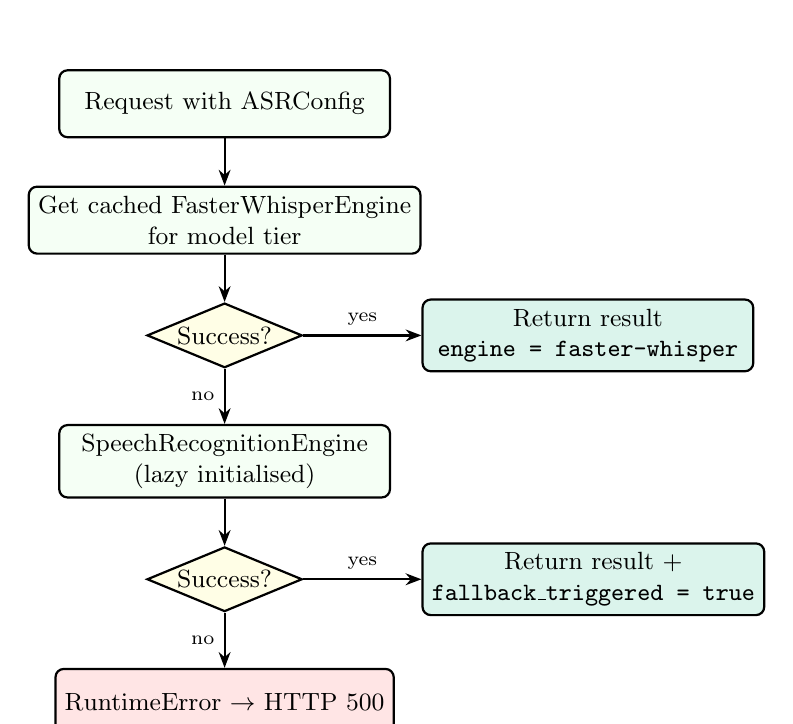
\begin{tikzpicture}[
  box/.style={draw, thick, rounded corners=3pt, fill=green!4, minimum width=4.2cm, minimum height=0.85cm, font=\small, align=center},
  dec/.style={draw, thick, diamond, aspect=2.4, fill=yellow!10, font=\small, align=center, inner sep=1pt},
  arr/.style={-{Stealth[length=2mm]}, thick}
]
\node[box] (in) {Request with ASRConfig};
\node[box, below=0.6cm of in] (c) {Get cached FasterWhisperEngine\\for model tier};
\node[dec, below=0.6cm of c] (ok) {Success?};
\node[box, right=1.5cm of ok, fill=emerald!15] (r1) {Return result\\\texttt{engine = faster-whisper}};
\node[box, below=0.7cm of ok] (sr) {SpeechRecognitionEngine\\(lazy initialised)};
\node[dec, below=0.6cm of sr] (ok2) {Success?};
\node[box, right=1.5cm of ok2, fill=emerald!15] (r2) {Return result +\\\texttt{fallback\_triggered = true}};
\node[box, below=0.7cm of ok2, fill=red!10] (err) {RuntimeError $\rightarrow$ HTTP 500};
\draw[arr] (in) -- (c); \draw[arr] (c) -- (ok);
\draw[arr] (ok) -- node[above,font=\scriptsize]{yes} (r1);
\draw[arr] (ok) -- node[left,font=\scriptsize]{no} (sr);
\draw[arr] (sr) -- (ok2);
\draw[arr] (ok2) -- node[above,font=\scriptsize]{yes} (r2);
\draw[arr] (ok2) -- node[left,font=\scriptsize]{no} (err);
\end{tikzpicture}
\caption{Primary/fallback decision flow inside \texttt{UnifiedASREngine}}
\end{figure}

%==================================================
% 7. TECHNOLOGY STACK
%==================================================
\section{Technology Stack \& Dependencies}
Comprehensive summary of the software packages, libraries and frameworks used (minimum versions are taken from \texttt{requirements.txt} and \texttt{frontend/package.json}):

\begin{tabularx}{\textwidth}{|L{2.9cm}|L{3.4cm}|L{1.7cm}|Y|}
\hline
\headrow \thc{Subsystem} & \thc{Technology / Library} & \thc{Version} & \thc{Role \& Engineering Purpose} \\ \hline
Backend Runtime & Python & 3.10+ & Core language for API, engine, CLI and tests \\ \hline
Web Framework & FastAPI & $\geq$0.100 & Async REST endpoints, validation, OpenAPI/Swagger docs \\ \hline
ASGI Server & Uvicorn & $\geq$0.22 & High-performance server hosting the FastAPI app \\ \hline
Multipart Parser & python-multipart & $\geq$0.0.6 & Parsing uploaded audio files in form-data requests \\ \hline
ASR Engine & Faster-Whisper & $\geq$1.0 & CTranslate2 Whisper inference with int8 quantisation \\ \hline
Tensor Runtime & PyTorch & $\geq$2.0 & Deep learning runtime used by the VAD/ASR stack \\ \hline
Fallback ASR & SpeechRecognition & $\geq$3.10 & Secondary engine used when Whisper is unavailable \\ \hline
Audio I/O & SoundFile & $\geq$0.12 & Decoding audio files into float32 arrays \\ \hline
Signal Processing & SciPy / NumPy & $\geq$1.10 / 1.24 & Resampling, normalisation, RMS and peak metrics \\ \hline
Frontend Library & React & 19.2 & Component-based single-page user interface \\ \hline
Build Tool & Vite & 8.x & Dev server (port 3000), hot reload, production build \\ \hline
Icons & lucide-react & 1.x & Vector icons for controls and cards \\ \hline
Audio Visualiser & Web Audio API / Canvas & W3C & Live frequency bars via \texttt{AnalyserNode} \\ \hline
Recording & MediaRecorder API & W3C & Capturing microphone audio in the browser \\ \hline
Linting & oxlint & 1.x & Fast JavaScript/JSX static analysis \\ \hline
Testing & PyTest / HTTPX & $\geq$7.4 / 0.24 & Unit and API integration tests via \texttt{TestClient} \\ \hline
\end{tabularx}

\subsection{Whisper Model Tiers}
\begin{tabularx}{\textwidth}{|L{2.4cm}|L{2.6cm}|Y|}
\hline
\headrow \thc{Model} & \thc{Parameters} & \thc{Typical Use} \\ \hline
tiny & $\sim$39 M & Fastest; quick drafts and low-end hardware \\ \hline
base (default) & $\sim$74 M & Best balance of speed and accuracy on CPU \\ \hline
small & $\sim$244 M & Better accuracy for accented or noisy speech \\ \hline
medium & $\sim$769 M & High accuracy; slower on CPU \\ \hline
large-v3 & $\sim$1550 M & Highest accuracy; GPU recommended \\ \hline
\end{tabularx}

%==================================================
% 8. DATA SCHEMA
%==================================================
\section{Data Model \& Configuration Schema}
ASR Studio is a stateless service: it does not keep a database. Every request is self-contained, uploaded audio is written to a temporary file, processed, and deleted in a \texttt{finally} block. The data model therefore consists of the configuration object passed to the engine and the structured JSON result returned to the client.

\subsection{ASRConfig Dataclass (\texttt{config.py})}
\begin{tabularx}{\textwidth}{|L{3.2cm}|L{2.6cm}|L{2.4cm}|Y|}
\hline
\headrow \thc{Field} & \thc{Type} & \thc{Default} & \thc{Description} \\ \hline
model\_size & ModelSize enum & base & Whisper tier: tiny, base, small, medium, large-v3 \\ \hline
device & str & cpu & Inference device: cpu or cuda \\ \hline
compute\_type & ComputeType enum & int8 & float32, float16, int8, int8\_float16 \\ \hline
task & TaskType enum & transcribe & transcribe or translate (to English) \\ \hline
language & Optional[str] & None & ISO code, None = auto-detect \\ \hline
beam\_size & int & 5 & Beam search width (API allows 1--10) \\ \hline
vad\_filter & bool & True & Enable Silero voice activity detection \\ \hline
word\_timestamps & bool & True & Return per-word start/end/probability \\ \hline
sample\_rate & int & 16000 & Target sampling rate in Hz \\ \hline
temperature & float & 0.0 & Decoding temperature (0 = greedy/beam) \\ \hline
initial\_prompt & Optional[str] & None & Optional context prompt for decoding \\ \hline
\end{tabularx}

\subsection{Transcription Result Schema}
\begin{tabularx}{\textwidth}{|L{4.2cm}|L{2.4cm}|Y|}
\hline
\headrow \thc{Field} & \thc{Type} & \thc{Description} \\ \hline
filename & string & Original uploaded file name \\ \hline
text & string & Full transcript (segments joined by spaces) \\ \hline
language & string & Detected or forced ISO language code \\ \hline
language\_probability & float & Confidence of language detection (0--1) \\ \hline
duration\_seconds & float & Length of the audio in seconds \\ \hline
processing\_time\_seconds & float & Wall-clock inference time \\ \hline
engine & string & \texttt{faster-whisper} or \texttt{speech-recognition-fallback} \\ \hline
model\_size & string & Model tier used \\ \hline
segments[] & array & id, start, end, text, confidence, words[] \\ \hline
segments[].words[] & array & word, start, end, probability \\ \hline
fallback\_triggered & bool & Present only when the fallback engine was used \\ \hline
fallback\_reason & string & Error message from the primary engine \\ \hline
\end{tabularx}

Segment confidence is derived from Whisper's average log-probability: $\text{confidence} = e^{\overline{\log p}}$, rounded to three decimals.

%==================================================
% 9. API ENDPOINTS
%==================================================
\section{REST API Resource Endpoints}
\begin{tabularx}{\textwidth}{|L{3.6cm}|L{1.5cm}|Y|}
\hline
\headrow \thc{Endpoint} & \thc{Method} & \thc{Description} \\ \hline
\texttt{/} & GET & Service name, author, version, status and documentation links \\ \hline
\texttt{/health} & GET & Health check returning \texttt{\{"status": "healthy"\}} \\ \hline
\texttt{/models} & GET & Available Whisper tiers, supported languages and default model \\ \hline
\texttt{/audio-info} & POST & Audio metrics: samples, sample rate, duration, RMS, peak, is\_silent \\ \hline
\texttt{/synthesize-sample} & POST & Generates a synthetic 1--10\,s 16\,kHz PCM WAV for benchmarking \\ \hline
\texttt{/transcribe} & POST & Transcribes/translates audio and returns the JSON result \\ \hline
\texttt{/transcribe/export} & POST & Transcribes and streams a downloadable .srt/.vtt/.txt/.json/.csv file \\ \hline
\texttt{/docs}, \texttt{/redoc} & GET & Interactive Swagger UI and ReDoc OpenAPI documentation \\ \hline
\end{tabularx}

\subsection{Query Parameters of \texttt{/transcribe}}
\begin{tabularx}{\textwidth}{|L{3.2cm}|L{2.2cm}|L{2.2cm}|Y|}
\hline
\headrow \thc{Parameter} & \thc{Type} & \thc{Default} & \thc{Validation / Meaning} \\ \hline
model & enum & base & tiny | base | small | medium | large-v3 \\ \hline
task & enum & transcribe & transcribe | translate \\ \hline
language & string & auto & ISO code or omitted for detection \\ \hline
beam\_size & int & 5 & $1 \le$ beam\_size $\le 10$ \\ \hline
vad\_filter & bool & true & Enable Silero VAD \\ \hline
word\_timestamps & bool & true & Include word-level timing \\ \hline
\end{tabularx}

\subsection{Request / Response Example}
\begin{lstlisting}[style=json]
// Request: POST /transcribe?model=base&task=transcribe
// Content-Type: multipart/form-data   [file=@speech_sample.wav]

// Response (200 OK)
{
  "filename": "speech_sample.wav",
  "text": "Welcome to the Automatic Speech Recognition Studio demonstration.",
  "language": "en",
  "language_probability": 0.985,
  "duration_seconds": 3.42,
  "processing_time_seconds": 0.284,
  "engine": "faster-whisper",
  "model_size": "base",
  "segments": [
    { "id": 0, "start": 0.0, "end": 3.42,
      "text": "Welcome to the Automatic Speech Recognition Studio demonstration.",
      "confidence": 0.98,
      "words": [
        { "word": "Welcome", "start": 0.0,  "end": 0.42, "probability": 0.99 },
        { "word": "to",      "start": 0.44, "end": 0.58, "probability": 0.99 } ] } ]
}
\end{lstlisting}
\textit{Values are illustrative; the field names match the backend implementation exactly.}

Validation failures (e.g.\ an unknown model name) are rejected by FastAPI with HTTP 422; unreadable audio returns HTTP 400 from \texttt{/audio-info}, and inference errors return HTTP 500 with a descriptive \texttt{detail} message.

%==================================================
% 10. MODULE BREAKDOWN
%==================================================
\section{Module Breakdown \& Implementation Details}
The code base is organised into decoupled modules:

\begin{itemize}[leftmargin=1.2em]
  \item \textbf{asr\_tool/api.py:} FastAPI application. Registers CORS middleware, creates one shared \texttt{UnifiedASREngine}, and defines the seven endpoints. Uploaded files are written to a \texttt{NamedTemporaryFile} with the original extension and always removed in a \texttt{finally} block.
  \item \textbf{asr\_tool/config.py:} Enumerations (\texttt{ModelSize}, \texttt{ComputeType}, \texttt{TaskType}, \texttt{OutputFormat}), the \texttt{SUPPORTED\_LANGUAGES} map and the \texttt{ASRConfig} dataclass with a \texttt{to\_dict()} serialiser.
  \item \textbf{asr\_tool/audio\_processor.py:} \texttt{AudioProcessor} with \texttt{load\_audio} (decode, mono down-mix, resample, normalise), \texttt{get\_audio\_info} (metrics), \texttt{create\_synthetic\_speech\_wav} and \texttt{save\_wav}.
  \item \textbf{asr\_tool/engine.py:} Abstract \texttt{BaseASREngine}, \texttt{FasterWhisperEngine} (lazy model loading, segment/word extraction, confidence), \texttt{SpeechRecognitionEngine} (fallback) and \texttt{UnifiedASREngine} (per-tier cache + fallback).
  \item \textbf{asr\_tool/exporters.py:} \texttt{TranscriptExporter} with SRT/VTT timecode formatters and \texttt{to\_txt/to\_srt/to\_vtt/to\_json/to\_csv/export\_to\_file}.
  \item \textbf{asr\_tool/cli.py:} \texttt{argparse} CLI with \texttt{transcribe}, \texttt{info} and \texttt{generate-sample} sub-commands, including recursive directory batch mode.
  \item \textbf{frontend/src/App.jsx:} The complete React studio (about 1,000 lines): state management with hooks, recording and visualiser, API calls, results viewer, benchmark, batch queue, API docs and theme switcher.
  \item \textbf{frontend/src/index.css:} Design system with CSS custom properties for the five themes, glassmorphism cards and responsive layout.
  \item \textbf{frontend/vite.config.js:} Dev server on port 3000 with a \texttt{/api} proxy to \texttt{127.0.0.1:8000}.
  \item \textbf{tests/:} Five PyTest modules covering API, audio processor, CLI, engine and exporters.
  \item \textbf{generate\_sample\_audio.py:} Helper script that creates sample audio for manual testing.
\end{itemize}

\subsection{Audio Preprocessing Algorithm}
\begin{lstlisting}[style=py]
audio, sr = sf.read(path, dtype="float32")          # 1. decode
if audio.ndim > 1:                                   # 2. stereo -> mono
    audio = np.mean(audio, axis=1)
if sr != 16000:                                      # 3. resample to 16 kHz
    n = int(len(audio) * 16000 / sr)
    audio = signal.resample(audio, n).astype(np.float32)
peak = np.max(np.abs(audio))                         # 4. peak normalise
if peak > 0:
    audio = audio / peak
\end{lstlisting}

The signal metrics are computed as
\[
\text{RMS} = \sqrt{\frac{1}{N}\sum_{n=1}^{N} x[n]^2}, \qquad
\text{Peak} = \max_n |x[n]|, \qquad
\text{is\_silent} = (\text{RMS} < 10^{-4}).
\]

\subsection{Whisper Inference Pipeline}
Inside Faster-Whisper, the 16\,kHz waveform is split into 30-second windows and converted into an 80-channel log-Mel spectrogram (25\,ms window, 10\,ms hop). The Transformer encoder turns the spectrogram into contextual audio embeddings; the decoder then generates text tokens autoregressively using cross-attention over those embeddings. Special tokens control the task (\texttt{<|transcribe|>} or \texttt{<|translate|>}), the language and timestamp prediction. Beam search keeps the \texttt{beam\_size} most probable hypotheses at every step. When \texttt{vad\_filter} is enabled, Silero VAD first removes non-speech regions, which reduces both runtime and hallucinated text on silence.

\begin{lstlisting}[style=py]
segments_raw, info = self.model.transcribe(
    audio_path, beam_size=cfg.beam_size, task=cfg.task.value,
    language=cfg.language, vad_filter=cfg.vad_filter,
    word_timestamps=cfg.word_timestamps,
    temperature=cfg.temperature, initial_prompt=cfg.initial_prompt)

for idx, seg in enumerate(segments_raw):
    confidence = round(float(np.exp(seg.avg_logprob)), 3)
    segments.append({"id": idx, "start": round(seg.start, 3),
                     "end": round(seg.end, 3), "text": seg.text.strip(),
                     "confidence": confidence, "words": words_list})
\end{lstlisting}

\subsection{Subtitle Timecode Formatting}
SRT and VTT differ only in the header and in the millisecond separator:
\begin{lstlisting}[style=py]
millis = int(round((seconds % 1) * 1000))
hrs, mins, secs = int(seconds)//3600, (int(seconds)//60) % 60, int(seconds) % 60
srt = f"{hrs:02d}:{mins:02d}:{secs:02d},{millis:03d}"   # 00:00:03,420
vtt = f"{hrs:02d}:{mins:02d}:{secs:02d}.{millis:03d}"   # 00:00:03.420
\end{lstlisting}

\begin{minipage}[t]{0.48\textwidth}
\textbf{Sample .srt output}
\begin{lstlisting}[style=base]
1
00:00:00,000 --> 00:00:03,420
Welcome to the Automatic Speech
Recognition Studio demonstration.
\end{lstlisting}
\end{minipage}\hfill
\begin{minipage}[t]{0.48\textwidth}
\textbf{Sample .vtt output}
\begin{lstlisting}[style=base]
WEBVTT

00:00:00.000 --> 00:00:03.420
Welcome to the Automatic Speech
Recognition Studio demonstration.
\end{lstlisting}
\end{minipage}

\subsection{Synthetic Speech Signal}
For benchmarking without real recordings, a 440\,Hz carrier is amplitude-modulated at a 3\,Hz ``syllable rate'' and mixed with light Gaussian noise:
\[
s(t) = \sin(2\pi \cdot 440\,t)\cdot \tfrac{1}{2}\bigl(1+\sin(2\pi \cdot 3\,t)\bigr) + \mathcal{N}(0,\,0.02^2)
\]
The signal is normalised and stored as 16-bit mono PCM at 16\,kHz.

%==================================================
% 11. UI WALKTHROUGH
%==================================================
\clearpage
\section{User Interface Walkthrough}
\subsection{Studio Landing Page \& Model Configuration}
On opening \texttt{http://localhost:3000}, the user sees the hero banner with capability badges, the theme selector, and four navigation tabs. The default \emph{Studio Audio Transcribe} tab shows the Model Configuration panel on the left (model tier, transcribe/translate toggle, source language, beam size slider, VAD and word-timestamp switches) and the audio source card on the right with \emph{Upload File} and \emph{Live Mic} modes.

\screenshot{figures/studio.png}{0.78\textwidth}{ASR Studio main interface with Model Configuration panel and audio source selector (Emerald Matrix theme)}

\subsection{Audio Upload, Live Recording \& Signal Analysis}
Dropping a file or finishing a recording immediately calls \texttt{POST /audio-info}; the returned duration, sample rate, RMS energy and peak amplitude are shown as metric cards together with an HTML5 audio player. During live recording, the canvas visualiser draws 64 frequency bars from the microphone stream at the browser's animation frame rate, and a timer shows the elapsed recording time.


\subsection{Transcription Results \& Export Hub}
Clicking \emph{Transcribe} sends the file and the selected settings to \texttt{POST /transcribe}. The results area displays the full transcript with a copy button, metadata cards (language and probability, duration, processing time, engine), the timed segment list with confidence scores, and five download buttons (TXT, SRT, VTT, JSON, CSV) which call \texttt{/transcribe/export}.

\screenshot{figures/results.png}{0.78\textwidth}{Transcription results with timed segments, confidence scores and export buttons}

\subsection{Synthetic Speech Benchmark}
The \emph{Synthetic Benchmark} tab lets the evaluator choose a signal duration (1--10\,s), generate the test WAV through \texttt{/synthesize-sample}, play it back, and run it through the full transcription pipeline. The measured processing time and real-time factor are displayed, allowing a quick check of performance on any machine without needing a recorded voice file.

\screenshot{figures/benchmark.png}{0.72\textwidth}{Synthetic speech generator and latency benchmark tab}


\subsection{Batch Processing Queue}
The \emph{Batch Processing Queue} tab accepts multiple files at once. They are transcribed one after another with the current model settings; a progress bar and per-file status cards (pending, processing, done, error) give live feedback, and each finished card shows the transcript preview.

\screenshot{figures/batch.png}{0.72\textwidth}{Batch processing queue for multi-file transcription}

\subsection{REST API \& CLI Documentation Tab}
The final tab documents every endpoint and CLI command with copy-ready examples, so developers can integrate ASR Studio into their own scripts or applications.

\screenshot{figures/api.png}{0.72\textwidth}{In-app REST API and CLI reference}


\subsection{Dynamic Theme Engine}
Themes are implemented with CSS custom properties scoped by a \texttt{data-theme} attribute on the root \texttt{<html>} element. Selecting a theme in the dropdown updates this attribute through a React \texttt{useEffect} hook, and every component re-colours instantly without reloading.

\screenshot{figures/theme_frost.png}{0.72\textwidth}{The same studio rendered with the Nordic Frost theme}

\begin{tabularx}{\textwidth}{|L{4.3cm}|Y|}
\hline
\headrow \thc{Theme} & \thc{Visual Character} \\ \hline
Emerald Matrix / Dark Velvet & Default; deep green background with emerald accents \\ \hline
Cyber Obsidian & Near-black surfaces with neon cyan highlights \\ \hline
Deep Nebula / Aurora & Purple-violet gradients \\ \hline
Tokyo Sunset / Horizon & Warm orange and pink tones \\ \hline
Nordic Frost / Minimal & Light, minimal palette for bright environments \\ \hline
\end{tabularx}

%==================================================
% 12. CLI + 13. INSTALLATION
%==================================================
\section{Command-Line Interface}
The same engine can be used without the browser through \texttt{python -m asr\_tool.cli}:

\begin{tabularx}{\textwidth}{|L{3.3cm}|Y|}
\hline
\headrow \thc{Sub-command} & \thc{Purpose and Key Options} \\ \hline
\texttt{transcribe} & File or directory (recursive) input; \texttt{-m} model, \texttt{-f} txt/srt/vtt/json/csv/all, \texttt{-l} language, \texttt{-t} transcribe/translate, \texttt{-o} output dir, \texttt{--device} cpu/cuda, \texttt{--beam-size} \\ \hline
\texttt{info} & Prints sample count, sample rate, duration, RMS, peak and silence flag \\ \hline
\texttt{generate-sample} & Writes a synthetic test WAV; \texttt{-d} duration in seconds \\ \hline
\end{tabularx}

\begin{lstlisting}[style=sh]
# Transcribe one file and export every format
python -m asr_tool.cli transcribe lecture.mp3 -m small -f all -o output/

# Translate a whole folder of Hindi audio into English subtitles
python -m asr_tool.cli transcribe recordings/ -l hi -t translate -f srt

# Inspect an audio file / create a test signal
python -m asr_tool.cli info lecture.mp3
python -m asr_tool.cli generate-sample sample.wav -d 5
\end{lstlisting}

\section{Installation \& Deployment Guide}
\textbf{Prerequisites:} Python 3.10+, Node.js 18+ with npm, Git, and a modern browser (Chrome, Edge or Firefox) with microphone permission. FFmpeg is recommended for compressed formats.

\begin{lstlisting}[style=sh]
# Step 1: Clone the repository
git clone https://github.com/Rajan3103/asr-studio.git
cd asr-studio

# Step 2: Create and activate a virtual environment
python -m venv .venv
.venv\Scripts\activate          # Windows
source .venv/bin/activate       # Linux / macOS

# Step 3: Install backend dependencies
pip install -r requirements.txt

# Step 4: Start the FastAPI backend (http://localhost:8000)
uvicorn asr_tool.api:app --host 0.0.0.0 --port 8000 --reload

# Step 5: In a second terminal, install and start the frontend
cd frontend
npm install
npm run dev                     # opens http://localhost:3000

# Step 6 (optional): run the test suite
pytest tests/ -v
\end{lstlisting}
On first use of a model tier, Faster-Whisper downloads the converted weights once and caches them locally; all later runs of that tier work offline.

%==================================================
% 14. TESTING
%==================================================
\clearpage
\section{Testing \& Quality Assurance}
ASR Studio includes 20 automated tests written with PyTest. API tests use FastAPI's \texttt{TestClient} (built on HTTPX), and audio tests generate their own synthetic WAV files in temporary directories, so the suite needs no external fixtures.

\begin{longtable}{|L{4.6cm}|L{3.0cm}|p{6.2cm}|L{1.4cm}|}
\hline
\headrow \thc{Test Identifier} & \thc{Target Component} & \thc{Validation Scenario} & \thc{Result} \\ \hline
\endhead
test\_root\_endpoint & API (GET /) & Status ``online'' and service metadata & PASSED \\ \hline
test\_health\_endpoint & API (GET /health) & Returns status ``healthy'' & PASSED \\ \hline
test\_models\_endpoint & API (GET /models) & Lists model tiers and languages & PASSED \\ \hline
test\_transcribe\_endpoint & API (POST /transcribe) & Synthetic WAV returns text, segments, engine & PASSED \\ \hline
test\_transcribe\_export\_endpoint & API (/transcribe/export) & Returns downloadable subtitle file & PASSED \\ \hline
test\_create\_synthetic\_speech\_wav & AudioProcessor & WAV file created with correct format & PASSED \\ \hline
test\_load\_audio & AudioProcessor & Mono float32 output at 16\,kHz & PASSED \\ \hline
test\_get\_audio\_info & AudioProcessor & Duration, RMS and peak computed correctly & PASSED \\ \hline
test\_save\_wav & AudioProcessor & 16-bit PCM WAV written and readable & PASSED \\ \hline
test\_cli\_parser\_build & CLI & Sub-commands and options parsed & PASSED \\ \hline
test\_cli\_generate\_sample & CLI & generate-sample writes a WAV file & PASSED \\ \hline
test\_cli\_info & CLI & info prints audio metrics & PASSED \\ \hline
test\_speech\_recognition\_engine\_fallback & Engine & Fallback engine returns valid structure & PASSED \\ \hline
test\_unified\_asr\_engine\_transcribe & Engine & Unified engine returns full result schema & PASSED \\ \hline
test\_to\_txt & Exporter & Plain text output & PASSED \\ \hline
test\_to\_srt & Exporter & SRT numbering and \texttt{,} timecodes & PASSED \\ \hline
test\_to\_vtt & Exporter & WEBVTT header and \texttt{.} timecodes & PASSED \\ \hline
test\_to\_json & Exporter & Valid, round-trippable JSON & PASSED \\ \hline
test\_to\_csv & Exporter & Header row and segment rows & PASSED \\ \hline
test\_export\_to\_file & Exporter & File written for the requested format & PASSED \\ \hline
\end{longtable}

\textbf{Test execution command:} \texttt{pytest tests/ -v} \quad (Result: 20 passed)

\subsection{Manual \& Integration Testing}
\begin{itemize}[leftmargin=1.2em,itemsep=1pt]
  \item Uploaded each supported format (WAV, MP3, FLAC, M4A, AAC, OGG) and verified metrics and transcripts.
  \item Recorded live speech in Chrome and Edge and checked visualiser, timer and transcription.
  \item Opened generated .srt and .vtt files in VLC Media Player to confirm subtitle timing.
  \item Imported .csv exports into a spreadsheet to verify column layout.
  \item Tested translate mode with non-English speech and auto language detection.
  \item Verified that invalid parameters (e.g.\ \texttt{beam\_size=20}) are rejected with HTTP 422.
\end{itemize}

%==================================================
% 15. PERFORMANCE + 16. SECURITY
%==================================================
\section{Performance Metrics \& Benchmarks}
Performance is reported using the \emph{Real-Time Factor} (RTF), the ratio of processing time to audio duration:
\[
\text{RTF} = \frac{T_{\text{processing}}}{T_{\text{audio}}}, \qquad \text{Speed-up} = \frac{1}{\text{RTF}}
\]
An RTF below 1.0 means the audio is transcribed faster than real time.

% >>> Fill in the values you measure with the Synthetic Benchmark tab or the CLI
% >>> (processing_time_seconds / duration_seconds). Replace "--" with your numbers.
\begin{tabularx}{\textwidth}{|L{4.0cm}|L{3.0cm}|Y|}
\hline
\headrow \thc{Metric Dimension} & \thc{Observed Value} & \thc{How It Was Measured} \\ \hline
RTF -- tiny (int8, CPU) & -- & 60\,s English speech clip, beam size 5 \\ \hline
RTF -- base (int8, CPU) & -- & Same clip, default settings \\ \hline
RTF -- small (int8, CPU) & -- & Same clip \\ \hline
First-request model load (base) & -- & Time of first \texttt{/transcribe} call after server start \\ \hline
Cached request overhead & -- & Repeated call minus inference time \\ \hline
Server RAM (base loaded) & -- & Task Manager / \texttt{htop} \\ \hline
Test hardware & -- & CPU model, cores, RAM \\ \hline
\end{tabularx}

\subsection{Factors Affecting Performance}
\begin{itemize}[leftmargin=1.2em,itemsep=1pt]
  \item \textbf{Model size:} larger tiers improve accuracy but increase latency and memory roughly in proportion to parameter count.
  \item \textbf{int8 quantisation:} stores weights in 8 bits, cutting memory use and speeding up CPU matrix multiplication with minimal accuracy loss.
  \item \textbf{Model caching:} the first request loads the model from disk; subsequent requests reuse the cached instance.
  \item \textbf{VAD filtering:} skipping silence reduces the amount of audio the decoder must process.
  \item \textbf{Beam size:} a smaller beam is faster; a larger beam can improve accuracy on difficult audio.
\end{itemize}

\section{Security \& Privacy Considerations}
\begin{itemize}[leftmargin=1.2em]
  \item \textbf{On-Device Primary Inference:} with Faster-Whisper, audio is processed entirely on the host machine; no audio is sent to an external service.
  \item \textbf{Fallback Transparency:} the secondary SpeechRecognition engine uses the online Google Web Speech service. It runs only if Whisper fails, and the response then carries \texttt{fallback\_triggered} and \texttt{fallback\_reason} so the user knows. Privacy-critical deployments can disable this fallback.
  \item \textbf{Ephemeral Storage:} uploaded audio is saved to a temporary file only for the duration of the request and deleted in a \texttt{finally} block, even when processing fails.
  \item \textbf{Input Validation:} enum-typed and range-checked query parameters prevent invalid model names or beam sizes from reaching the engine.
  \item \textbf{Browser Sandboxing:} microphone capture requires explicit user permission through the browser.
  \item \textbf{Deployment Hardening:} CORS is currently open (\texttt{allow\_origins=["*"]}) for local development; production deployments should restrict origins, add authentication, enforce upload size limits and serve over HTTPS.
\end{itemize}

%==================================================
% 17. COMPARISON + 18. FUTURE
%==================================================
\section{Comparison with Commercial Solutions}
Feature matrix comparing ASR Studio with widely used transcription services (pricing and features as publicly listed; they change over time):

\begin{tabularx}{\textwidth}{|L{3.0cm}|Y|Y|Y|Y|}
\hline
\headrow \thc{Dimension} & \thc{ASR Studio} & \thc{Otter.ai} & \thc{Google Cloud STT} & \thc{AWS Transcribe} \\ \hline
Hosting & On-device & Cloud & Cloud & Cloud \\ \hline
Cost & Free, open source (MIT) & Subscription & Pay per minute & Pay per minute \\ \hline
Offline use & Yes (primary engine) & No & No & No \\ \hline
Speech translation to English & Built in & Limited & Separate API & Separate service \\ \hline
SRT / VTT export & Built in & Paid plans & Manual & Yes \\ \hline
Model choice & 5 tiers & Fixed & Several & Fixed \\ \hline
Self-hostable API & Yes & No & No & No \\ \hline
Speaker diarisation & Not yet & Yes & Yes & Yes \\ \hline
\end{tabularx}

\section{Limitations}
\begin{itemize}[leftmargin=1.2em,itemsep=1pt]
  \item Transcription happens after recording stops; there is no live word-by-word streaming yet.
  \item No speaker diarisation, so multi-speaker recordings are not labelled per speaker.
  \item Large models (medium, large-v3) are slow on CPU-only machines.
  \item The export endpoint re-runs transcription instead of reusing the previous result.
  \item No user accounts or transcript history; results are not stored on the server.
\end{itemize}

\section{Future Enhancements}
\begin{itemize}[leftmargin=1.2em]
  \item \textbf{Real-Time Streaming:} WebSocket endpoint feeding audio chunks to the model for live captions.
  \item \textbf{Speaker Diarisation:} integrate pyannote.audio to label ``Speaker 1'', ``Speaker 2''.
  \item \textbf{Indian Language Focus:} fine-tuned models for Tamil, Hindi, Telugu and code-mixed speech.
  \item \textbf{Result Caching:} hash uploaded audio and reuse results for exports.
  \item \textbf{Transcript History:} optional SQLite/PostgreSQL storage with search.
  \item \textbf{Containerised Deployment:} Docker images with GPU support for lab servers.
  \item \textbf{Summarisation:} optional local LLM to generate meeting notes or lecture summaries.
\end{itemize}

%==================================================
% 19. CONCLUSION & REFERENCES
%==================================================
\clearpage
\section{Conclusion \& References}
ASR Studio demonstrates that modern, open-source speech recognition can be packaged into a complete, user-friendly application that runs on everyday hardware. By combining Faster-Whisper's int8-quantised Transformer inference with a FastAPI microservice and a React studio interface, the project delivers accurate multilingual transcription, English translation, timed segments and five subtitle/export formats without depending on paid cloud APIs for its primary path. The modular design -- separate preprocessing, engine, exporter, API and CLI layers -- keeps the code testable, as shown by the 20 passing automated tests, and makes the engine reusable from a browser, a script or another service.

\subsection*{Key Technical Milestones Achieved}
\begin{itemize}[leftmargin=1.2em,itemsep=1pt]
  \item[$\blacksquare$] On-device Whisper inference with int8 CPU quantisation and per-tier model caching.
  \item[$\blacksquare$] Unified audio pipeline converting six formats and live recordings into 16\,kHz mono signals.
  \item[$\blacksquare$] Graceful engine fallback with transparent reporting.
  \item[$\blacksquare$] TXT, SRT, VTT, JSON and CSV export from both the web studio and the CLI.
  \item[$\blacksquare$] React studio with live visualiser, benchmark, batch queue and five themes.
\end{itemize}

\subsection*{References}
\begin{enumerate}[leftmargin=1.5em,itemsep=2pt]
  \item Radford, A., Kim, J.~W., Xu, T., Brockman, G., McLeavey, C., \& Sutskever, I. (2022). \textit{Robust Speech Recognition via Large-Scale Weak Supervision}. arXiv:2212.04356.
  \item Vaswani, A., et al. (2017). \textit{Attention Is All You Need}. Advances in Neural Information Processing Systems (NeurIPS).
  \item Klein, G., et al. (2020). \textit{Efficient and High-Quality Neural Machine Translation with OpenNMT}. Proc. Workshop on Neural Generation and Translation. (CTranslate2 inference engine.)
  \item SYSTRAN. \textit{faster-whisper: Faster Whisper transcription with CTranslate2}. \url{https://github.com/SYSTRAN/faster-whisper}
  \item Silero Team. \textit{Silero VAD: pre-trained enterprise-grade Voice Activity Detector}. \url{https://github.com/snakers4/silero-vad}
  \item Ram\'irez, S. \textit{FastAPI Documentation}. \url{https://fastapi.tiangolo.com}
  \item W3C. \textit{Web Audio API} and \textit{MediaStream Recording} specifications.
  \item Meta Open Source. \textit{React Documentation}. \url{https://react.dev}
\end{enumerate}

\subsection*{Project Links}
\textbf{GitHub Repository:} \url{https://github.com/Rajan3103/asr-studio}\\
\textbf{Video Presentation:} \url{https://drive.google.com/file/d/19zCYGW_cIZd9RbbAUSxV_bN3umef547Z/view?usp=sharing}

\vspace{1cm}
\begin{center}
{\bfseries DEPARTMENT OF COMPUTER SCIENCE AND ENGINEERING}\\
{\bfseries SRM INSTITUTE OF SCIENCE AND TECHNOLOGY, TIRUCHIRAPPALLI}
\end{center}

\end{document}
